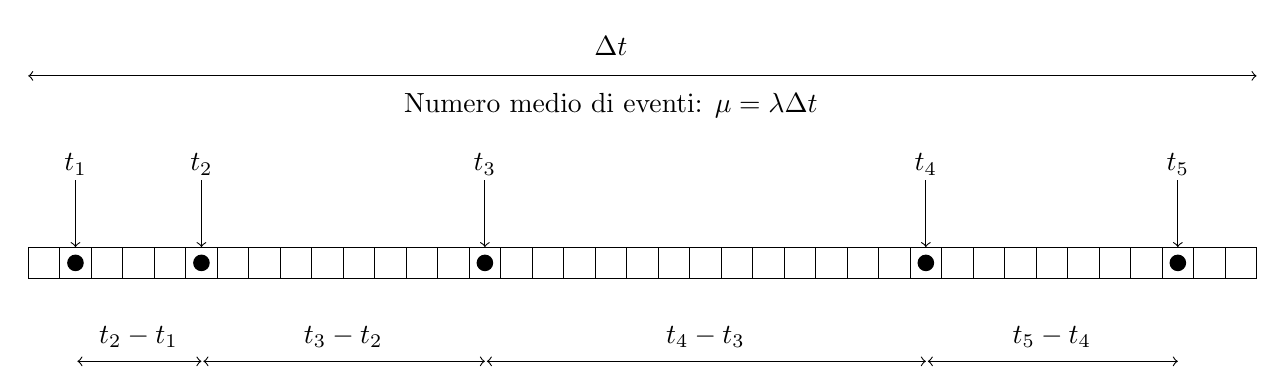
\begin{tikzpicture}[main node/.style={rectangle,draw,minimum size=4mm}]%
  \pgfmathsetmacro{\xscale}{0.4}
  \pgfmathsetmacro{\yscale}{1.25}
  \foreach \x in {1,...,39}
  \node[main node] at (\x*\xscale, 0) {};
  \foreach \e[count=\xi from 1] in {2,6,15,29,37} {
    \fill (\e*\xscale, 0) circle [radius=3pt];
    \node (e) at (\e*\xscale, \yscale) {$t_\xi$};
    \draw [out=-90,in=90,-{>[scale=1.8]}] (\e*\xscale, \yscale-0.5*\xscale) to (\e*\xscale, 0.5*\xscale);
  }
  \draw [out=0,in=180,{<[scale=1.8]}-{>[scale=1.8]}] (0.5*\xscale,1.9*\yscale) to (39.5*\xscale,1.9*\yscale);
  \node at (19*\xscale,2.2*\yscale) {$\Delta t$};
  \node at (19*\xscale,1.6*\yscale) {Numero medio di eventi: $\mu = \lambda \Delta t$};
  
  \node[inner sep=0pt] (e) at (2*\xscale, -1*\yscale) {};
  \foreach \e[count=\xi from 1] in {6,15,29,37} {
    \draw [out=0,in=180,{<[scale=1.8]}-{>[scale=1.8]}] (e) to (\e*\xscale, -1*\yscale);
    \node[inner sep=0pt] (e) at (\e*\xscale, -1*\yscale) {};
  }
  \node at (4*\xscale,-0.75*\yscale) {$t_2 - t_1$};
  \node at (10.5*\xscale,-0.75*\yscale) {$t_3 - t_2$};
  \node at (22*\xscale,-0.75*\yscale) {$t_4 - t_3$};
  \node at (33*\xscale,-0.75*\yscale) {$t_5 - t_4$};
\end{tikzpicture}
